\chapter{量子网络望远镜}
\label{chap:17}

\begin{chapteropening}
量子网络望远镜针对的是长基线光学干涉的一个具体工程瓶颈：弱星光的单光子相干态很难在公里到百公里尺度上低损耗、低相位噪声地传到同一个合束器。量子方案把要长距离传输的对象从未知星光改成可预先制备、可验证、可丢弃重来的纠缠资源；星光到达后，只在本地与量子存储或辅助光子相互作用，再用经典通信合并测量结果。Gottesman-Jennewein-Croke 的量子中继望远镜、Khabiboulline-Borregaard-De Greve-Lukin 的存储型光学量子网络，以及 Stas 等的非局域光学干涉实验，把这个方向从理论资源估算推进到实验原型 \citep{2012PhRvL.109g0503G,2019PhRvL.123g0504K,2026Natur.651..326S,2026PhRvA.113a2608P,2025PhRvR...7d3278Z,2023PhRvL.130p0801M}。
\end{chapteropening}

\section{为什么传统光学合束会卡在长基线}

先把问题说成最小模型：不是“量子网络让望远镜更灵敏”，而是“怎样在不长距离搬运未知星光的情况下保留一阶相干相位”。双望远镜振幅干涉测的是复可见度；它和天空亮度的 Fourier 关系已经在第 \ref{chap:05} 章式 \eqref{eq:ch05-vcz} 中给出。量子网络方案关心的是极弱星光：每个相干时间窗里的平均光子数 \(\epsilon\ll1\)，绝大多数时间窗是空的，少数时间窗只含一个来自天体的光子。若这个光子在到达探测器前没有被路径信息破坏，它不是“已经属于左望远镜”或“已经属于右望远镜”的经典标签，而是左右两条接收路径的叠加。单个点源在两孔径上的一光子态可写成
\begin{equation}
  |\psi_\star\rangle
  =
  \frac{|1\rangle_L|0\rangle_R
  +
  e^{i\phi}
  |0\rangle_L|1\rangle_R}{\sqrt2},
  \qquad
  \phi
  =
  \frac{2\pi{\bf B}\cdot\boldsymbol\theta}{\lambda}.
  \label{eq:ch17-stellar-single-photon}
\end{equation}
\begin{formulaexplain}[公式 (17.1) 解读]
\(|\psi_\star\rangle\) 是单个星光光子在左右孔径之间的路径叠加态，\(\phi\) 是由基线 \({\bf B}\)、源角位置 \(\boldsymbol\theta\) 和波长 \(\lambda\) 决定的几何相位。振幅干涉要保住的正是这个相位。
\end{formulaexplain}
这里的 \(|1\rangle_L|0\rangle_R\) 表示该时间窗里左空间模式有一个光子、右空间模式为空，\(|0\rangle_L|1\rangle_R\) 表示相反情形。\(\phi\) 是几何相位，\({\bf B}\) 是投影基线，\(\boldsymbol\theta\) 是点源相对相位中心的角位置，\(\lambda\) 是波长。扩展源可以看成许多点源相位的非相干混合；混合后保留下来的正是复可见度 \(V\)，对应的单光子密度矩阵为
\begin{equation}
  \rho_1
  =
  \frac{1}{2}
  \begin{pmatrix}
  1 & V\\
  V^* & 1
  \end{pmatrix}_{\{|10\rangle,|01\rangle\}} .
  \label{eq:ch17-single-photon-density}
\end{equation}
\begin{formulaexplain}[公式 (17.2) 解读]
\(\rho_1\) 是单光子子空间的密度矩阵，非对角元 \(V\) 是复可见度。对角元只说明光子可在任一望远镜出现，非对角元才保存源的相干相位和结构信息。
\end{formulaexplain}
普通振幅干涉要把这两个空间模式送到同一个 beamsplitter。若其中一路经过长度 \(L\) 的有损链路，单光子透过率常写成
\begin{equation}
  \eta_{\rm ch}(L)
  =
  10^{-\alpha_{\rm dB}L/10}.
  \label{eq:ch17-link-loss}
\end{equation}
\begin{formulaexplain}[公式 (17.3) 解读]
\(\eta_{\rm ch}\) 是链路透过率，\(\alpha_{\rm dB}\) 是每公里 dB 损耗，\(L\) 是传输距离。dB 损耗会指数式吞掉未知星光，这是长基线直接光学合束的核心瓶颈。
\end{formulaexplain}
\(\alpha_{\rm dB}\) 的单位是 \({\rm dB\,km^{-1}}\)。可见光在普通光纤中可到 \(20-30\,{\rm dB\,km^{-1}}\) 的量级，\(1\,{\rm km}\) 就只剩 \(10^{-2}\) 到 \(10^{-3}\) 以下；1550 nm telecom fiber 可低到 \(\sim0.2\,{\rm dB\,km^{-1}}\)，但星光频率转换、耦合、相位稳定和背景噪声会把理想透过率再乘上效率因子；晴空自由空间链路可用 \(\sim0.5\,{\rm dB\,km^{-1}}\) 作量级估算，但大气湍流和指向误差不是单纯指数损耗 \citep{2012PhRvL.109g0503G,2019PhRvL.123g0504K,2024SPIE13095E..1NR}。

\begin{figure}[tbp]
\centering
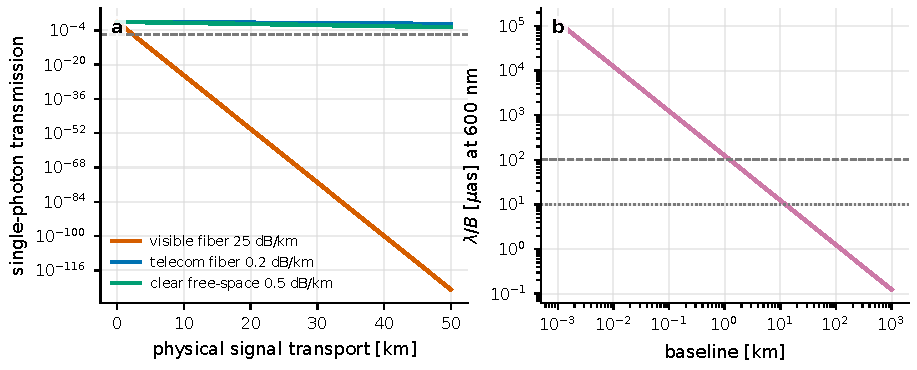
\includegraphics[width=0.94\linewidth]{figures/generated/chapter_17/ch17_architecture_loss.pdf}
\caption{长基线的吸引力和困难来自同一个量纲。左图把直接传输单光子星光的几种链路损耗画成透过率；可见光光纤在公里尺度已经严重衰减，telecom fiber 也会在百公里尺度变得昂贵。右图给出 \(\lambda/B\) 的角分辨率标度；600 nm 光在 1 km 基线达到百微角秒量级，100 km 基线进入微角秒量级。}
\label{fig:ch17-architecture-loss}
\end{figure}

角分辨率的基本标度是
\begin{equation}
  \theta_{\rm res}
  \sim
  \frac{\lambda}{B}
  =
  124\,\mu{\rm as}
  \left(\frac{\lambda}{600\,{\rm nm}}\right)
  \left(\frac{1\,{\rm km}}{B}\right).
  \label{eq:ch17-resolution-scale}
\end{equation}
\begin{formulaexplain}[公式 (17.4) 解读]
\(\theta_{\rm res}\) 是干涉角分辨率标度，\(B\) 是基线长度。基线越长，分辨率越高；量子网络方案追求的是在不传输未知星光的情况下把 \(B\) 推到 km 甚至更长。
\end{formulaexplain}
\(B=10\,{\rm km}\) 时是 \(12\,\mu{\rm as}\)，\(B=100\,{\rm km}\) 时是 \(1.2\,\mu{\rm as}\)。量子网络望远镜的吸引力就在这个尺度上：它不一定提高单孔径灵敏度，却可能把光学/近红外干涉从几百米推向 km、十 km 或更远的基线。HBT 强度干涉已经绕开了光学相位传输，但它主要给 \(|V|^2\)，灵敏度和相位恢复路线不同；量子网络路线的目标是保留一阶相干的相位信息，同时不把未知星光长距离搬运 \citep{1956Natur.178.1046H,2014A&G....55c3.28K,2016OptL...41.1094K,2023OExpr..3144246C,2024SPIE13095E..1NR}。

\section{预共享纠缠怎样替代传星光}

Gottesman-Jennewein-Croke 方案用一个已知的路径纠缠“实验室光子”
\begin{equation}
  |\Phi_\delta\rangle
  =
  \frac{|1\rangle_L|0\rangle_R
  +
  e^{i\delta}
  |0\rangle_L|1\rangle_R}{\sqrt2}
  \label{eq:ch17-lab-entangled-photon}
\end{equation}
\begin{formulaexplain}[公式 (17.5) 解读]
\(|\Phi_\delta\rangle\) 是预共享实验室路径纠缠光子，\(\delta\) 是可控相位。它替代了长距离搬运未知星光的任务：纠缠资源可以提前制备、验证，失败则丢弃重来。
\end{formulaexplain}
与未知星光光子做本地干涉。纠缠态可以提前通过量子网络分发；若分发失败，就重新来一次，不损失星光。星光到达后，两端各自把星光模式和实验室模式送入本地 beamsplitter，并只保留左右两边各探测到一个光子的事件。相关和反相关点击概率含有
\begin{equation}
  P_{\pm}(\delta)
  =
  \frac{1}{2}
  \left[
  1
  \pm
  {\rm Re}
  \left(
  V e^{-i\delta}
  \right)
  \right].
  \label{eq:ch17-gjc-probability}
\end{equation}
\begin{formulaexplain}[公式 (17.6) 解读]
\(P_\pm(\delta)\) 是两类符合点击概率，\(V\) 是星光复可见度，\(\delta\) 是实验室纠缠相位。改变 \(\delta\) 就像扫描参考相位，可以从点击率振荡中读出 \(V\) 的实部和虚部。
\end{formulaexplain}
扫描或改变 \(\delta\) 就可估计 \(V\) 的实部和虚部。这里的本地 beamsplitter 和符合探测相当于一次 Bell 态投影：星光模式和实验室纠缠模式的哪一路信息被擦除，只剩两条路径的相位关系。Bell 态测量就是把两个光子投影到一组最大纠缠的两模基上。线性光学只能无歧义地区分其中一部分点击组合，所以只有约一半有效星光事件进入估计；若能做完整 Bell 态测量或使用更复杂的量子处理，这个 \(50\%\) 损失可在原则上避免 \citep{1982Natur.299..802W,1993PhRvL..70.1895B,2012PhRvL.109g0503G}。

资源率是这条路线的第一道限制。若观测带宽是 \(\Delta\nu\)，相干时间约 \(1/\Delta\nu\)。直接 GJC 路线需要在每个可能有星光的相干时间窗准备匹配的纠缠光子；\(\Delta\nu=10\,{\rm GHz}\) 意味着每秒 \(10^{10}\) 个时间窗。Rajagopal 等给出的天文路线图指出，当前高质量 entangled-photon source 的典型速率距离这个数很远；GJC 更适合作为短基线 on-sky proof of principle，短期内还难以替代现有光学干涉阵列 \citep{2024SPIE13095E..1NR,2012PhRvL.109g0503G}。

Khabiboulline-Borregaard-De Greve-Lukin 方案利用弱光源的事实：每个长测量窗口内平均只有 \(\epsilon\ll1\) 个相关星光光子。把窗口分成 \(M\sim1/\epsilon\) 个 time bins 后，只有一个 time bin 可能含有光子。若用 unary code，需要 \(M\) 个 Bell pairs；若用 binary code，存下到达时间只需
\begin{equation}
  n_{\rm mem}
  =
  \left\lceil
  \log_2(M+1)
  \right\rceil
  \simeq
  \left\lceil
  \log_2(1/\epsilon)
  \right\rceil
  \label{eq:ch17-binary-timebin}
\end{equation}
\begin{formulaexplain}[公式 (17.7) 解读]
\(n_{\rm mem}\) 是需要的存储 qubit 数，\(M\) 是 time bins 数，\(\epsilon\) 是每个 bin 的平均星光光子数。弱光的稀疏性把资源从 \(M\) 个纠缠对降到 \(\log_2M\) 个存储位。
\end{formulaexplain}
个 memory qubits，每个 qubit pair 用一个 Bell pair 做非局域 parity check。若 \(M=10^6\)，约 20 个 qubits 就能编码到达时间，而 unary code 需要一百万个纠缠对。论文中的代表性量级是：对 \(\Delta f=1\,{\rm MHz}\)、1 s 测量窗口，\(N=10^6\) 个 time bins 对应 \(\log_2N\simeq20\)；在一个天文例子中，10 等星、\(10\,{\rm m^2}\) 收集面积和 \(10\,{\rm GHz}\) 检测带宽可导出约 \(20-30\) 个 qubits 与 \(\sim200\,{\rm kHz}\) 纠缠供应率的资源目标。Stas 等的补充分析也用 \(20\) 个 SiV 节点、1 kHz 零距离 entanglement rate 和 1 s 窗口展示了这种对数缩放的路径 \citep{2019PhRvL.123g0504K,2022PhRvA.106c2424C,2026Natur.651..326S,2024SPIE13095E..1NR}。

\begin{figure}[tbp]
\centering
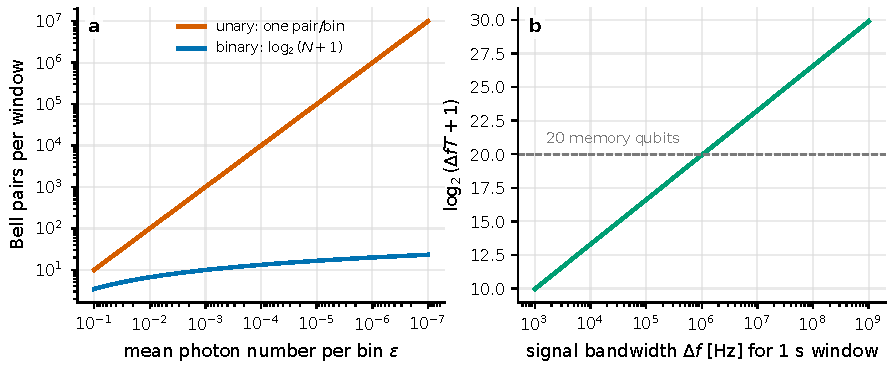
\includegraphics[width=0.94\linewidth]{figures/generated/chapter_17/ch17_timebin_scaling.pdf}
\caption{弱星光使 time-bin 编码有意义。左图比较 unary code 和 binary code 对 Bell pairs 的需求：当每个 bin 的平均光子数 \(\epsilon\) 很小，\(M\sim1/\epsilon\) 个 bin 可被 \(\log_2(M+1)\) 个 memory qubits 标记。右图显示 1 s 测量窗口中，1 MHz 带宽对应约 \(10^6\) 个 bin，也就是约 20 个 qubits。}
\label{fig:ch17-timebin}
\end{figure}

量子中继是这些方案的底层通信技术。直接传未知量子态受损耗和不可克隆定理限制；中继把总距离分段，先在短段内建立纠缠，再通过 entanglement swapping 连接长距离。理想中继可把指数损耗变成更温和的资源缩放，但真实系统还要面对 Bell-state measurement 成功率、memory lifetime、dark counts、gate fidelity 和 frequency conversion。DLCZ 原子系综协议、量子互联网路线和量子存储综述都把存储放在资源预算中心，因为它负责把概率成功事件同步起来 \citep{1998PhRvL..81.5932B,2001Natur.414..413D,2011RvMP...83...33S,2008Natur.453.1023K,2012IEEEN..26d..59V,2006quant.ph..7182U}。

\section{资源率、存储时间和保真度怎样闭合}

任何量子网络望远镜方案最后都要回到同一张账本。角分辨率由 \(B\) 给出，但能不能观测由资源率、存储时间、保真度和星光事件率共同决定；少一个环节，长基线的相位杠杆就无法兑现。第一个资源约束是纠缠供应率。若被接受的星光事件率是 \(R_\star\)，每个事件平均消耗 \(n_{\rm pair}\) 个 Bell pairs，则
\begin{equation}
  R_{\rm ent}
  \gtrsim
  \frac{n_{\rm pair}R_\star}{p_{\rm ready}},
  \label{eq:ch17-entanglement-rate}
\end{equation}
\begin{formulaexplain}[公式 (17.8) 解读]
\(R_{\rm ent}\) 是所需纠缠供应率，\(R_\star\) 是有效星光事件率，\(n_{\rm pair}\) 是每个事件消耗的 Bell pairs 数，\(p_{\rm ready}\) 是资源已就绪概率。它把天文事件率直接转成量子网络吞吐量要求。
\end{formulaexplain}
\(p_{\rm ready}\) 是星光到达时可用 Bell pairs 已经准备好的概率。\(R_\star\) 指进入目标空间模式、频率通道、偏振通道、时间窗并通过质量筛选后的事件率，不等同于望远镜总 photon rate。对宽带亮源，\(R_\star\) 可非常高，GJC 型方案会被资源率压垮；对窄带弱源，\(R_\star\) 小，memory-assisted scheme 才有机会用较低 \(R_{\rm ent}\) 换取长基线。

第二个资源约束是存储时间。最低限度，量子态或测量记录要等到经典通信和非局域校验完成：
\begin{equation}
  T_{\rm mem}
  \gtrsim
  \max\!\left[
    \frac{B}{c},
    T_{\rm ent},
    T_{\rm proc},
    T_{\rm win}
  \right].
  \label{eq:ch17-memory-time}
\end{equation}
\begin{formulaexplain}[公式 (17.9) 解读]
\(T_{\rm mem}\) 是量子存储必须保持相干的时间，右边取基线光行时、纠缠生成时间、处理时间和观测窗口的最大值。真正限制存储的常常不是 \(B/c\)，而是同步和 time-bin 窗口。
\end{formulaexplain}
\(B/c=3.3\,\mu{\rm s}\,(B/{\rm km})\)。\(100\,{\rm km}\) 基线只需 \(0.33\,{\rm ms}\) 的光行时，但 Khabiboulline 型二进制 time-bin 方案还可能需要 \(T_{\rm win}\sim1\,{\rm s}\) 的测量窗口来覆盖窄带弱光；这比光行时要求严得多。量子存储文献通常用 fidelity、efficiency、storage time、bandwidth、multimode capacity 和 wavelength 六个指标描述硬件。单光子存储的 conditional fidelity 是读出的波包与写入波包的重合度，efficiency 是成功读出光子的概率；对未知光态 teleportation 或非局域干涉，二者的乘积、相位噪声和模式匹配都进入最终 visibility \citep{2009NaPho...3..706L,2010EPJD...58....1S,2016JMOp...63.2005H}。

\begin{figure}[tbp]
\centering
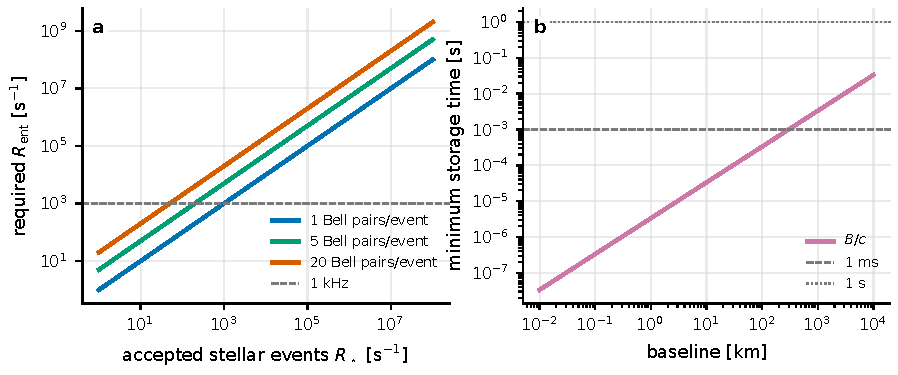
\includegraphics[width=0.94\linewidth]{figures/generated/chapter_17/ch17_entanglement_resources.pdf}
\caption{纠缠率和存储时间给出第一层资源闭合条件。左图把被接受的星光事件率 \(R_\star\) 转成 Bell pair rate；每个事件消耗的纠缠对越多，需求线越高。右图把基线转为 \(B/c\)；对 km 级基线，光行时是微秒到毫秒，但窄带存储方案常由测量窗口和纠缠生成时间决定。}
\label{fig:ch17-entanglement-resources}
\end{figure}

资源预算里常把链路中几个主要损失因子乘在一起，得到一个有效保真度标度：
\begin{equation}
  F_{\rm eff}
  \simeq
  F_{\rm Bell}
  \eta_{\rm write}
  \eta_{\rm read}
  \eta_{\rm conv}
  \exp(-T/T_2)
  (1-p_{\rm dark})
  M_{\rm mode}.
  \label{eq:ch17-effective-fidelity}
\end{equation}
\begin{formulaexplain}[公式 (17.10) 解读]
\(F_{\rm eff}\) 是粗略有效资源质量，包含 Bell pair 保真度、写入/读出效率、频率转换、存储退相干、暗触发和模式匹配。任何一项偏低都会乘法式降低最终可见度。
\end{formulaexplain}
\(F_{\rm Bell}\) 是预共享 Bell pair fidelity；\(\eta_{\rm write}\)、\(\eta_{\rm read}\) 是写入和读出效率；\(\eta_{\rm conv}\) 是频率转换效率；\(T_2\) 是相干时间；\(p_{\rm dark}\) 是等效暗触发概率；\(M_{\rm mode}\le1\) 表示频率、时间、偏振和空间模式匹配。这个式子不是完整量子信道模型，但它能快速暴露瓶颈。例如 \(T/T_2=1\) 单独就给 \(e^{-1}\simeq0.37\) 的相干因子；若 \(F_{\rm Bell}=0.8\)、读写各 \(0.7\)、转换 \(0.8\)，还没算暗计数和模式失配，乘积已降到 \(\sim0.3\)。

\begin{figure}[tbp]
\centering
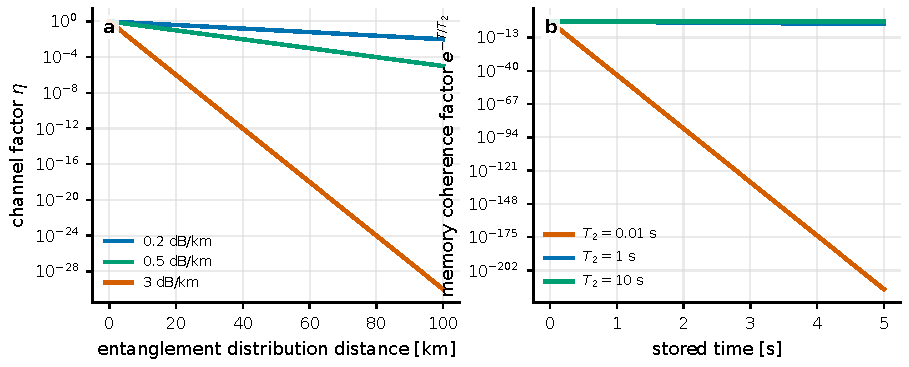
\includegraphics[width=0.94\linewidth]{figures/generated/chapter_17/ch17_fidelity_distance.pdf}
\caption{有效资源质量由链路和存储共同决定。左图显示不同 dB/km 损耗下的通道因子；右图显示存储时间与 \(T_2\) 的关系。一个长基线方案即使角分辨率诱人，也要让 Bell pair fidelity、读写效率、频率转换和存储相干同时闭合。}
\label{fig:ch17-fidelity-distance}
\end{figure}

频率转换是天文版本的额外难题。许多量子存储材料的强耦合频率不在目标天文波段；长距离光纤又偏好 telecom band。量子频率转换要在保持单光子相干、偏振或 time-bin 编码的同时降低噪声。若目标是和星光做干涉，转换后的谱宽、中心频率、时间波包和偏振都要和星光模式匹配；一个 \(1\%\) 的模式失配不会只损失 \(1\%\) 光子数，它会直接降低干涉 visibility \citep{1990OptL...15.1476K,2010EPJD...58....1S,2016JMOp...63.2005H,2024SPIE13095E..1NR}。

\section{连续变量和辅助单光子路线各解决什么}

前面的方案把路径自由度看成离散 qubit，并把时间窗或到达时间写进存储。还有两类互补想法：连续变量路线试图直接传送光场正交分量，辅助单光子路线则把可损失的实验室光子拿来承担长距离链路风险。它们解决的瓶颈不同，也带来不同资源成本。

这里的连续变量指光场的两个正交分量，而不是“左/右路径”这样的离散 qubit。连续变量 teleportation 用预共享的两模压缩真空态和本地测量，把一个模式的正交分量信息转移到远端模式。若资源态是
\begin{equation}
  |\psi_{\rm TMSV}\rangle
  =
  \sqrt{1-\lambda^2}
  \sum_{n=0}^{\infty}
  \lambda^n |n\rangle_A|n\rangle_B,
  \qquad
  \bar N = 2\sinh^2 r,
  \label{eq:ch17-tmsv}
\end{equation}
\begin{formulaexplain}[公式 (17.11) 解读]
\(|\psi_{\rm TMSV}\rangle\) 是两模压缩真空资源态，\(\lambda\) 或 \(r\) 控制压缩强度，\(\bar N\) 是总平均光子数。压缩越强，连续变量 teleportation 的附加噪声越小，但资源成本越高。
\end{formulaexplain}
\(r\) 是 squeezing parameter，\(\bar N\) 是两模总平均光子数。理想 \(r\to\infty\) 才能无噪声 teleport 任意连续变量态；有限 \(r\) 会加入等效高斯噪声，常按 \(e^{-2r}\) 标度下降。Gottesman 等已经指出，CV teleportation 可避免单 qubit Bell measurement 的 \(50\%\) 限制，但连续变量中继和远距离高保真压缩资源更难。最新 optimality 分析还提醒，比较不同资源态时要考虑 photon-number superselection rule、locality 和有限 entanglement budget；压缩度只是资源账本中的一项 \citep{1998PhRvL..80..869B,2012PhRvL.109g0503G,2025PhRvR...7d3278Z}。

另一条近中期路线不依赖长寿命量子存储，而是用本地或地面产生的单光子辅助星光干涉。Marchese-Kok 方案把星光光子尽早在接收端测量，让辅助单光子跨基线传输；损耗主要作用在“可重来的”地面光子上。对小角度位置估计，相位和角度满足
\begin{equation}
  \phi
  =
  \frac{2\pi B\theta}{\lambda},
  \qquad
  \sigma_\theta
  \ge
  \frac{\lambda}{2\pi B}
  \frac{1}{\sqrt{N_{\rm ev}\mathcal F_\phi}},
  \label{eq:ch17-angle-fisher}
\end{equation}
\begin{formulaexplain}[公式 (17.12) 解读]
\(\phi\) 是角位置 \(\theta\) 对应的干涉相位，\(\sigma_\theta\) 是角度误差下限，\(N_{\rm ev}\) 是有效事件数，\(\mathcal F_\phi\) 是单事件相位 Fisher 信息。基线越长、事件越多、单事件信息越高，定位越精。
\end{formulaexplain}
\(N_{\rm ev}\) 是有效事件数，\(\mathcal F_\phi\) 是单事件相位 Fisher 信息。Marchese-Kok 在 \(\lambda=628\,{\rm nm}\)、光纤 attenuation length \(L_0=10\,{\rm km}\) 的模型中得到十几 \(\mu{\rm as}\) 量级的定位标度；Modak-Kok 进一步指出，星光模式占据数 \(\epsilon\ll1\) 和辅助光子与星光的不可区分度会显著改变收益。若 \(\epsilon\) 从 1 降到 \(0.01\)，增加辅助光子数的优势会很快变弱；若模式不可区分度只有 \(96\%\)，三光子方案还可能有收益，但更高光子数不一定继续改善 \citep{2023PhRvL.130p0801M,2025PhRvA.111d3701M}。

Padilla、Sajjad、Saif 和 Guha 的分布式纠缠成像工作把这个问题推进到更一般的多模成像极限：先在每个接收站做本地空间模式排序，再用预共享 Bell pairs 模拟非局域 beamsplitter 或更一般的干涉网络。长基线只是资源的一部分；单孔径内的模式信息、源结构先验、阵列几何和测量基选择都会改变 Fisher 信息。对双星角分离，若只追求 Rayleigh 标度下的 \(\lambda/B\)，可能错过本地模式排序带来的小分离优势；若只追求本地 superresolution，又得不到长基线提供的相位杠杆 \citep{2026PhRvA.113a2608P,2025PhRvR...7d3278Z}。

\section{实验原型怎样转成误差预算}

实验原型的价值不只是证明“能纠缠两个远端节点”，而是给资源账本里的每一项填上可测数字。Stas 等的 2026 年实验把“非局域相位测量”从线路图推到实验台。他们用两个 SiV diamond nanocavity 节点、电子自旋和 \({}^{29}{\rm Si}\) nuclear-spin memory，先生成远程 Bell pair，再让弱信号光在本地与节点相互作用，通过 photon erasure 和非局域 non-destructive heralding 过滤真空事件。实验中 electron Bell state 可达 \(F=0.83(3)\)，entanglement rate 为 \(13\,{\rm Hz}\) 时 \(F\ge0.5\)，为 \(1.9\,{\rm Hz}\) 时 \(F=0.79(3)\)。完整非局域相位测量中，heralding 后 visibility 从无 heralding 的 \(0.031(18)\) 提高到 \(0.090(26)\)；加入 \(1.55\,{\rm km}\) 光纤基线后，nuclear parity oscillation visibility 为 \(0.11(4)\)，Bell pair fidelity 仍高于可验证纠缠阈值，约 \(F=0.63(3)\) \citep{2026Natur.651..326S}。

这类实验的相位误差由有效试验次数、herald 成功率和测得的相位振荡 visibility 共同决定。用 Fisher 信息表示时，
\begin{equation}
  \mathcal I_\phi
  \simeq
  N_{\rm tr}\,
  p_{\rm succ}\,
  V_{\rm meas}^2,
  \qquad
  {\rm Var}(\hat\phi)\ge \mathcal I_\phi^{-1}.
  \label{eq:ch17-fisher-visibility}
\end{equation}
\begin{formulaexplain}[公式 (17.13) 解读]
\(\mathcal I_\phi\) 是总相位 Fisher 信息，\(N_{\rm tr}\) 是试验次数，\(p_{\rm succ}\) 是 herald 成功率，\(V_{\rm meas}\) 是测得可见度。可见度以平方进入信息量，所以少量相干损失会明显放大相位误差。
\end{formulaexplain}
\(N_{\rm tr}\) 是 protocol trials 数，\(p_{\rm succ}\) 是成功 herald 的概率，\(V_{\rm meas}\) 是相位振荡 visibility。Stas 等给出的实现中
\begin{equation}
  p_{\rm succ}
  =
  \eta_{\rm erasure}\eta_{\rm herald}
  P(n_{\rm photon}\ge1),
  \label{eq:ch17-psucc}
\end{equation}
\begin{formulaexplain}[公式 (17.14) 解读]
\(p_{\rm succ}\) 是一次试验被接受的概率，包含 photon erasure、herald 探测和至少一个光子到达的概率。提高它不能只靠加大光强；多光子污染会降低 visibility，反而减少总 Fisher 信息。
\end{formulaexplain}
多光子事件、mis-heralding 和 Bell state infidelity 会降低 \(V_{\rm meas}\)。这解释了为什么“herald 成功率高”不一定好：若通过提高平均光子数获得更多 herald，却引入多光子污染，visibility 可能下降，\(\mathcal I_\phi\) 不升反降。相位误差再用式 \eqref{eq:ch17-angle-fisher} 转成角度误差；\(B\) 越长，相同 \(\sigma_\phi\) 对应越小 \(\sigma_\theta\)，但长基线也会增加 entanglement distribution overhead、相位锁定难度和延迟。

\begin{figure}[tbp]
\centering
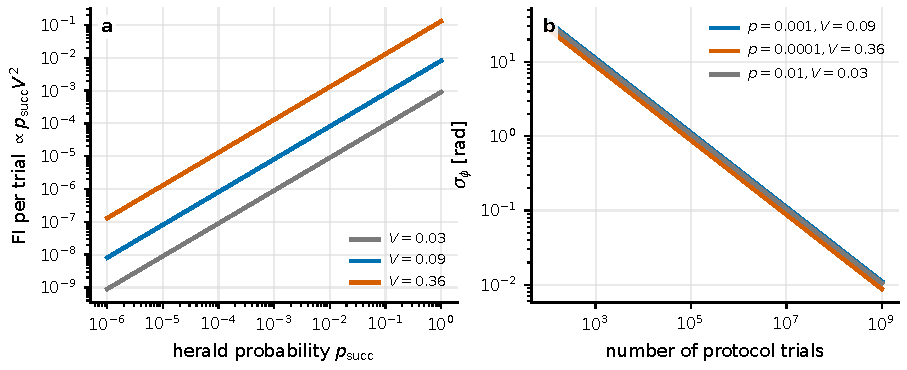
\includegraphics[width=0.94\linewidth]{figures/generated/chapter_17/ch17_fisher_visibility.pdf}
\caption{非局域相位测量的统计收益同时依赖成功概率和可见度。左图画出单 trial Fisher 信息的标度 \(p_{\rm succ}V^2\)；visibility 降低三倍，信息降低九倍。右图把 trial 数转成相位误差，显示高重复率、低 mis-herald 和高 Bell fidelity 要同时成立。}
\label{fig:ch17-fisher-visibility}
\end{figure}

Crawford 等的两光子精密天体测量实验提供了另一种近期台阶：用两个准热光源和时间标记探测器，在 benchtop analogue 中看到 photon-pair coincidence 随相位变化的相关行为。这个实验不等同于完整量子网络望远镜，但它很适合作为 on-sky 前的验证：时间标记、polarization matching、coherence time、HBT peak fitting、phase stability 和数据筛选都和真实天文弱光相关 \citep{2023OExpr..3144246C}。

把所有资源放在同一张图里，近期实验大致处在 \(R_{\rm ent}\sim1-10\,{\rm Hz}\)、短基线、低有效 visibility 区域；天文可用的 memory-assisted narrowband 方案可能需要 \(R_{\rm ent}\sim{\rm kHz}\) 到 \(100\,{\rm kHz}\)、\(T_{\rm mem}\sim{\rm ms}\) 到 s、几十个 memory qubits 和高模式匹配；宽带成像则更难。资源约束要一起闭合：\(R_{\rm ent}\) 不够会浪费星光事件，\(T_{\rm mem}\) 不够会让 parity check 赶不上，\(F_{\rm eff}\) 不够会洗掉 visibility，\(R_\star\) 估错会让整套方案在第一晚观测前就失去可行性。

\begin{figure}[tbp]
\centering
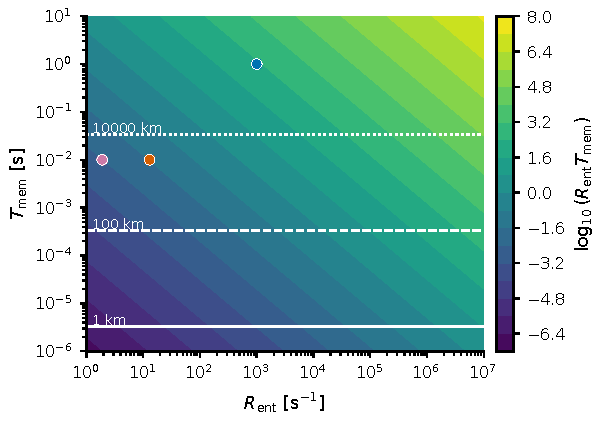
\includegraphics[width=0.94\linewidth]{figures/generated/chapter_17/ch17_network_parameter_space.pdf}
\caption{量子网络望远镜的资源空间由纠缠率和存储时间共同决定。白线标出 1 km、100 km 和 \(10^4\) km 基线的 \(B/c\) 时间；散点给出当前实验 Hz 级纠缠率和远期 kHz-s 级目标的量级。颜色只是资源乘积标度，完整可行性还要乘上 fidelity、模式匹配和天文光子率。}
\label{fig:ch17-network-space}
\end{figure}

\section{量子网络和强度干涉怎样互补}

量子网络望远镜不应被写成强度干涉的替代品，而应被写成长期互补路线。强度干涉已经能用本地时间标记和离线相关绕开光学相位传输，代价是主要得到 \(|V|^2\)；量子网络路线想保留一阶相干的相位信息，代价是要支付纠缠、存储、转换和 heralding 的资源账本。短期内仍要和 ELT、VLTI、CHARA、CTAO 或强度干涉阵列并行发展。近期目标是强度干涉和两光子相关：硬件接近已有大面积光收集器、SNSPD/SPAD 时间标记、窄带滤波和离线相关，科学目标集中在亮星角直径、双星和发射线区域。下一步加入本地模式排序、two-photon astrometry 和 GJC 型短基线 on-sky 演示，目标是证明星光模式可和实验室纠缠资源稳定干涉。memory-assisted 非局域一阶相干测量需要量子存储、频率转换、纠缠分发、Bell fidelity 和天文仪器同步共同成熟，应放在更远期的技术目标中 \citep{1956Natur.178.1046H,2023OExpr..3144246C,2024SPIE13095E..1NR,2026Natur.651..326S}。

\Needspace{11\baselineskip}
观测规划可以从一个简单闭合条件开始：
\begin{equation}
  N_{\rm useful}
  =
  R_\star T_{\rm obs}
  p_{\rm ready}
  p_{\rm succ}
  V_{\rm meas}^2
  \gtrsim
  N_{\rm req}(\sigma_\theta,{\bf B},\lambda).
  \label{eq:ch17-useful-events}
\end{equation}
\begin{formulaexplain}[公式 (17.15) 解读]
\(N_{\rm useful}\) 是真正有相位信息的有效事件数，等于星光事件率、观测时间、资源就绪概率、成功率和可见度平方的乘积。它必须超过目标精度所需的 \(N_{\rm req}\)，方案才有观测意义。
\end{formulaexplain}
\(T_{\rm obs}\) 是总观测时间；\(N_{\rm req}\) 由目标角精度、阵列几何和模型参数维数决定。这个式子把天文学和量子工程放在同一张账本上：亮源、窄带、已知到达时间或周期信号会降低资源压力；暗弱宽带连续源会把所有困难放大。同样的账本也适用于更一般的观测设计，只是可观测量从非局域相位换成 \(|V|^2\)、\(g^{(2)}\)、偏振角或时间延迟。

量子网络望远镜目前最有价值的是这张可行性账本，而不是某个已经成熟的仪器方案。下一部分回到观测设计：科学参数需要落到事件率、通道、基线、背景和协方差上，然后才谈得上选择强度干涉、偏振事件表、瞬变触发或未来非局域相位测量。

